\chapter{Umsetzung}
\label{umsetzung}

Dieses Kapitel beschreibt die konkrete Umsetzung des Chatbots für Freudenberg \& Co. KG (\ac{FCO}). 
Dabei wird auf die einzelnen technischen Schritte eingegangen, die für die Entwicklung und Implementierung des Chatbots erforderlich sind, einschließlich der Integration der ausgewählten Large Language Models und Embedding-Modelle.

\section{Umsetzung über SAP AI Core}

Die Implementierung des Chatbots, auch AI Assistant genannt, erfolgte unter Einsatz verschiedener Technologien und Komponenten. 
Eine der wichtigsten davon ist das Python SAP AI Core \ac{SDK}, welches eine reibungslose Integration des Chatbots mit SAP AI Core ermöglicht und die effiziente Übermittlung der Prompts an das Large Language Model (\ac{LLM}) gewährleistet.

Eine weitere zentrale Komponente ist die PostgreSQL-Datenbank, die als Hauptspeicherort für Metadaten und Vektoren dient. 
PostgreSQL wurde aufgrund seiner Stabilität, Skalierbarkeit und umfangreichen Unterstützung für komplexe Datenstrukturen gewählt, die für die effiziente Speicherung und Abfrage großer Mengen an Informationen erforderlich sind. 
Die Datenbank speichert Metadaten, die für die Verwaltung und das Retrieval von Dokumenten erforderlich sind, wie Kontext-ID, Dokument-ID und Dokumentname. 
Diese Metadaten ermöglichen es dem System, Dokumente effizient zu organisieren und zu referenzieren.

Darüber hinaus werden Vektoren in der Datenbank gespeichert, um eine semantische Suche innerhalb der eingebetteten Dokumente zu ermöglichen. 
Die Verwendung von Vektoren erlaubt es dem Chatbot, nicht nur wortgenaue Übereinstimmungen zu finden, sondern auch semantisch verwandte Inhalte zu identifizieren und so kontextbezogene Antworten zu generieren.

Die nächste Schlüsselkomponente in der Architektur ist LlamaIndex, das verwendet wird, um die eingebetteten Dokumente zu verwalten und die semantische Suche durchzuführen. 
LlamaIndex ermöglicht es, die in der PostgreSQL-Datenbank gespeicherten Vektoren effizient zu durchsuchen und die relevantesten \textit{chunks} eines Dokuments zu identifizieren. 
Diese werden in einer rangbasierten Reihenfolge zurückgegeben, basierend auf ihrer semantischen Relevanz zur gestellten Anfrage. 
LlamaIndex integriert sich dabei nahtlos mit dem \ac{LLM}, indem es die relevantesten Chunks zusammen mit dem Prompt an das Modell sendet, was zu präziseren und kontextbezogeneren Antworten führt.

Bei der Auswahl der Modelle für den AI Assistant war es entscheidend, nicht einfach die leistungsfähigsten Modelle zu verwenden. 
Da der Chatbot interne Daten verarbeitet, bestand die Anforderung, ausschließlich Open-Source-Modelle zu verwenden. Dies ist notwendig, um sicherzustellen, 
dass die sensiblen Firmendaten innerhalb der Freudenberg-Infrastruktur bleiben und nicht an externe Anbieter übertragen werden. 
Daher fiel die Wahl auf \textit{LLaMA3-70b}, das als bestes Open-Source-\ac{LLM} in der Untersuchung \ref{eval_llm} hervorging.
Dieses Modell bietet eine hohe Antwortqualität und ist gleichzeitig datenschutzkonform, da es lokal in der eigenen Cloud Foundry-Umgebung gehostet werden kann. 

Für die Einbettung der Dokumente wurde das \textit{multilingual-e5-large} Modell verwendet, da es das beste Open-Source-Embedding-Modell in der Untersuchung \ref{eval_embedding} war. 
Obwohl das Modell \textit{text-embedding-3-large} von OpenAI die besten Ergebnisse zeigte, konnte es aufgrund seiner proprietären Lizenz nicht eingesetzt werden. 
Die Entscheidung für \textit{multilingual-e5-large} stellt sicher, dass auch für die Embedding-Modelle die Datenschutzanforderungen und der Open-Source-Ansatz gewahrt bleiben. 
Dieses Modell erzeugt ebenfalls dichte Vektorrepräsentationen von Dokumenten, die anschließend in der semantischen Suche verwendet werden.

Für die Verarbeitung der Dokumente wurde eine \textit{chunk size} von 128 und ein \textit{top k}-Wert von 20 festgelegt. 
Diese Parameter wurden in der Evaluation für das Modell \textit{LLaMA3-70b} als optimal identifiziert, da sie die beste Balance zwischen Antwortqualität und Effizienz boten. 
Durch die Verwendung dieser Einstellungen kann der Chatbot relevante Textabschnitte aus den Dokumenten präzise identifizieren und dabei effizient arbeiten.

\section{AI Assistant Funktionalitäten}
\subsection{Erstellung einer neuen Anfrage}
Die erste Interaktion mit dem Chatbot beginnt auf der Startseite, auf der Nutzer bestehende Anfragen einsehen oder eine neue Anfrage erstellen können (siehe Abbildung \ref{fig:chatbot_start}). 
Es gibt zwei Arten von Anfragen: private und öffentliche Anfragen. Jede Anfrage, die ein Nutzer selbst erstellt, ist privat und nur für diesen Nutzer zugänglich. 
Admins haben jedoch die Möglichkeit, Anfragen mit vordefinierten Kontexten anzulegen, die als öffentlich markiert werden können. 
Öffentliche Anfragen stehen allen Nutzern zur Verfügung und ermöglichen es, auf bereits eingebettete Dokumente zuzugreifen und diese zu verwenden. 
Diese Funktion ist besonders nützlich für Abteilungen wie die Cyber Security- oder Rechtsabteilung, in denen die Mitarbeiter häufig auf dieselben Dokumente zugreifen müssen. 
Durch die öffentlichen Anfragen wird der Aufwand für die Mitarbeiter verringert, da sie nicht jedes Dokument selbst hochladen und einbetten müssen.

Die bereits erstellten Anfragen sind zusammen mit den zugehörigen Kontexten und Metadaten in der PostgreSQL-Datenbank gespeichert, um spätere Zugriffe auf dieselbe Anfrage zu ermöglichen.

\begin{figure}[H]
    \centering
    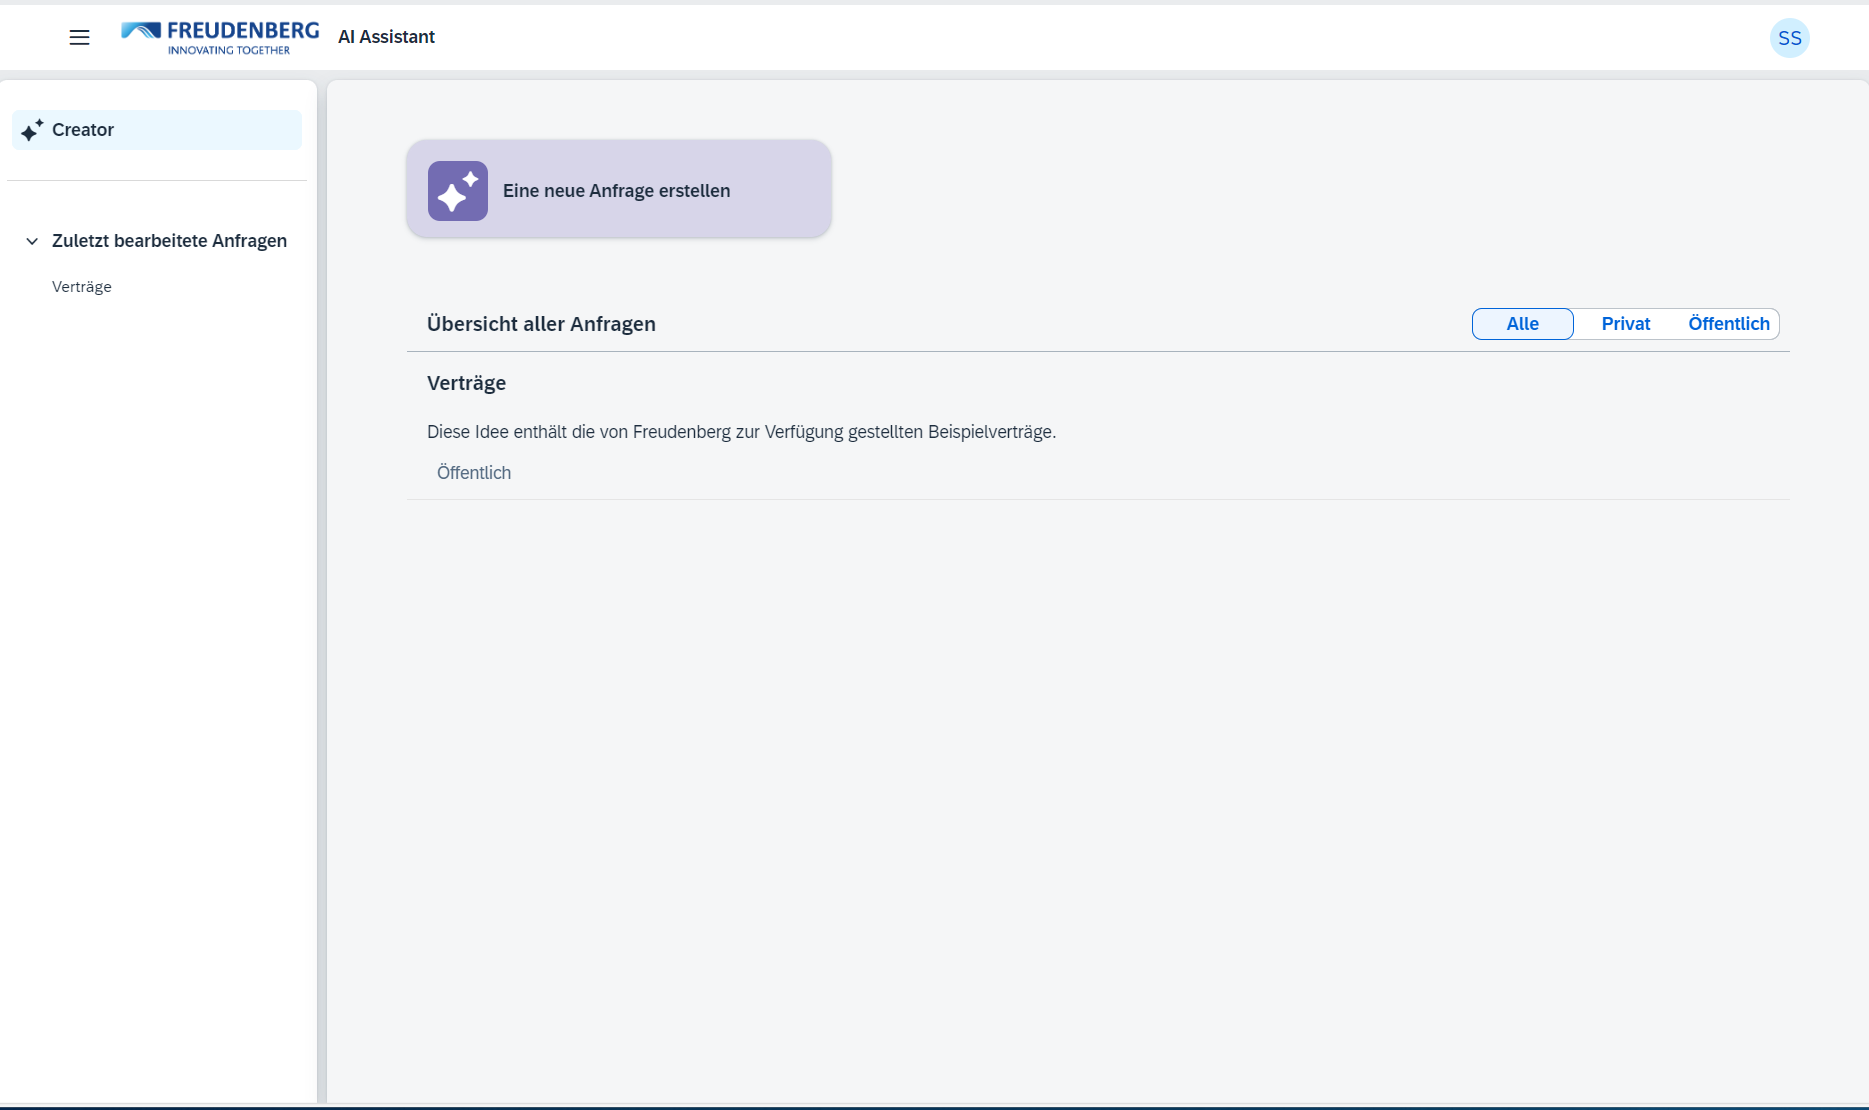
\includegraphics[width=1\textwidth]{img/Chatbot_start.png}
    \caption{AI Assistant Startseite}
    \label{fig:chatbot_start}
\end{figure}

Klickt der Benutzer auf „Eine neue Anfrage erstellen“, gelangt er zur Upload-Seite, auf der beliebig viele PDF-Dokumente hochgeladen werden können, 
die in den Kontext der Anfrage eingebunden werden (siehe Abbildung \ref{fig:neue_anfrage}). 

Im Hintergrund werden die hochgeladenen PDF-Dokumente zunächst in einem File Storage gespeichert. Ein PDF Reader liest dann die hochgeladenen Dateien aus und erstellt relevante Metadaten, 
wie die Kontext-ID und Dokument-ID. Diese Metadaten dienen dazu, die Dokumente zu verwalten und sie nach der Verarbeitung in Chunks korrekt zuzuweisen.

Nach der Extraktion der Metadaten werden die PDF-Dokumente in Chunks unterteilt. Diese Chunks werden dann durch das Embedding-Modell \textit{multilingual-e5-large} in Vektoren umgewandelt. 
Diese Vektoren werden anschließend in einer Vektor-Datenbank gespeichert, wobei sie mit der Kontext-ID verknüpft sind, um die Zuordnung der Chunks zu einem bestimmten Kontext zu gewährleisten. 
Die Vektor-Datenbank ermöglicht so die semantische Suche.

Sobald der Benutzer eine Anfrage an den Chatbot stellt, wird der Prompt zusammen mit der zugehörigen Kontext-ID abgesendet. 
LlamaIndex übernimmt dann die Verarbeitung des Prompts, nachdem dieser ebenfalls mithilfe des Embedding-Modells in einen Vektor umgewandelt wurde. 
Hierbei führt LlamaIndex eine Similarity-Suche in der Vektor-Datenbank durch, wobei nur die Einträge mit derselben Kontext-ID berücksichtigt werden. 
Auf diese Weise werden die am besten passenden Chunks der hochgeladenen Dokumente identifiziert.

Diese relevanten Chunks werden aus der Vektor-Datenbank geladen und zusammen mit dem Prompt über SAP AI Core an das \ac{LLM} \textit{LLaMA3-70b} gesendet. 
Die Verbindung zu SAP AI Core erfolgt über das Python SAP AI Core \ac{SDK}, das es ermöglicht, die Prompts und die Chunks effizient an das \ac{LLM} zu übermitteln. 
Das \ac{LLM} verarbeitet diese Informationen und generiert auf Basis des Prompts und der relevanten Chunks eine Antwort, die dann an den Benutzer zurückgegeben wird. 
Durch diesen Ablauf wird sichergestellt, dass der Chatbot nicht nur schnelle, sondern auch kontextuell passende und präzise Antworten liefern kann.


\begin{figure}[H]
    \centering
    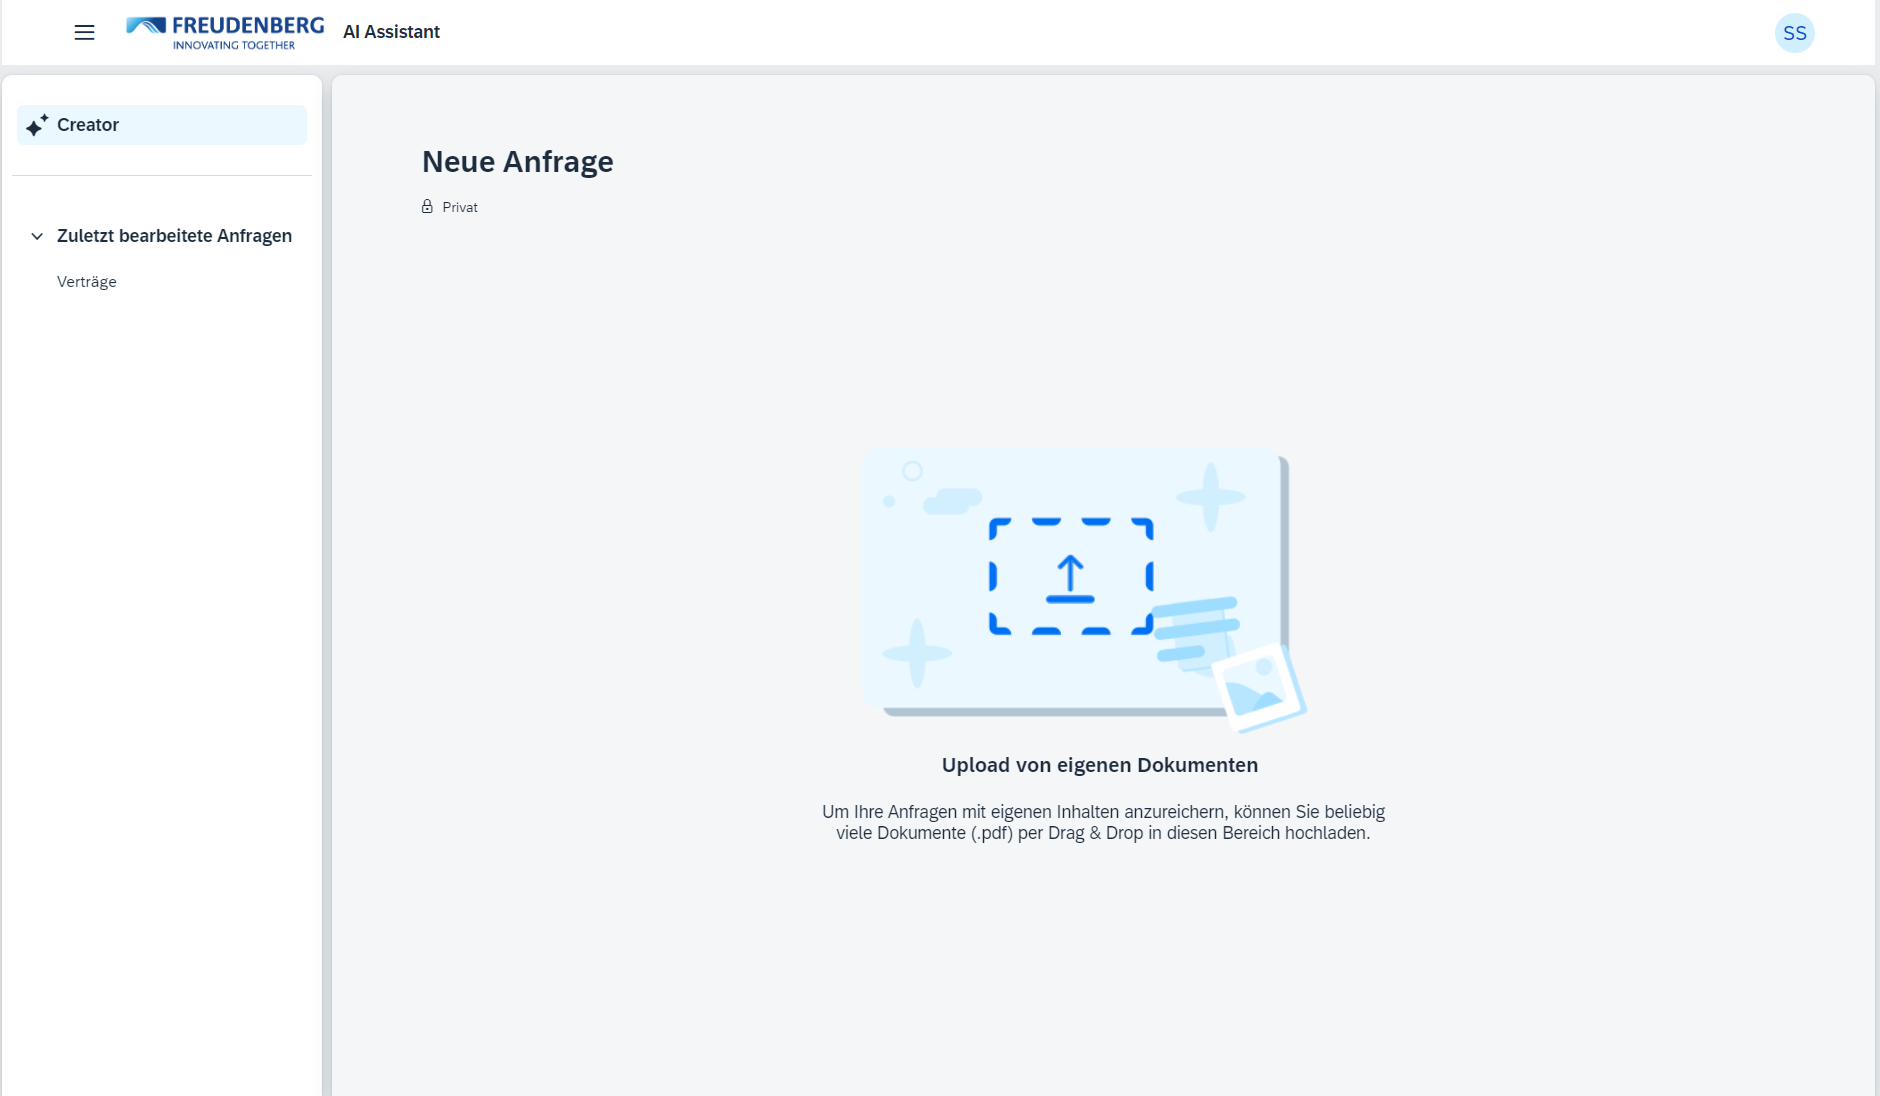
\includegraphics[width=1\textwidth]{img/Chatbot_neue_Anfrage.png}
    \caption{Eine neue Anfrage erstellen}
    \label{fig:neue_anfrage}
\end{figure}

\subsection{Zugriff auf bestehende Anfrage}

Außer eine neue Anfrage anzulegen kann der Benutzer auch auf bestehende Anfragen zugreifen, z. B. auf die öffentlich erstellte Anfrage „Verträge“ (siehe Abbildung \ref{fig:chatbot_vertraege_leer}). 
Der Kontext dieser Anfrage umfasst 12 Verträge der Freudenberg Gruppe, darunter \acp{NDA} und andere geschäftliche Verträge. Vertrauliche Daten in den Dokumenten wurden für die Arbeit geschwärzt. 

Diese Anfrage wurde vorab als Beispiel in den AI Assistant integriert, um den Benutzern die Möglichkeit zu geben, sich mit den Funktionen des Tools vertraut zu machen. 

\begin{figure}[H]
    \centering
    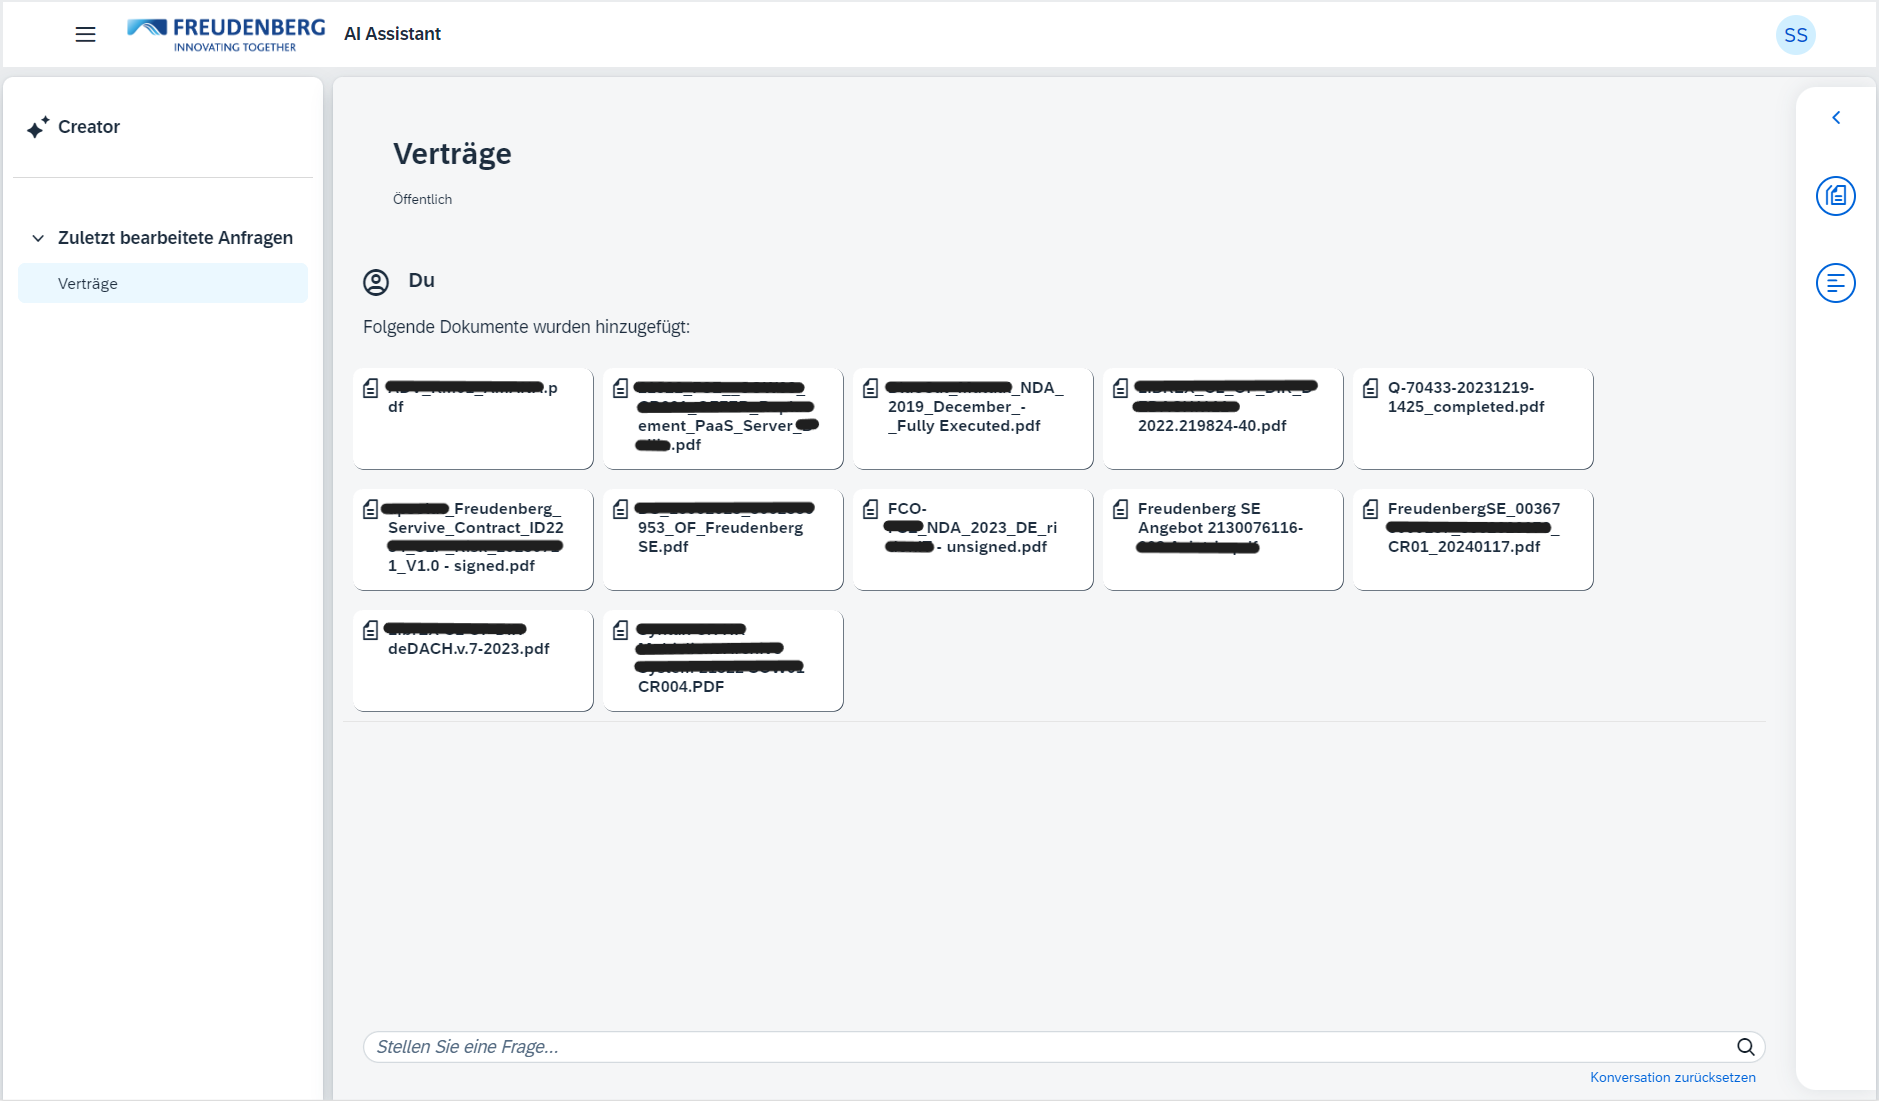
\includegraphics[width=1\textwidth]{img/Chatbot_vertraege_leer.png}
    \caption{Anfrage „Verträge“ mit vorbereitetem Kontext}
    \label{fig:chatbot_vertraege_leer}
\end{figure}

Benutzer können spezifische Fragen zu den Verträgen stellen, woraufhin der Chatbot den Prompt mithilfe des Embedding-Modells \textit{multilingual-e5-large} in einen Vektor umwandelt und zusammen mit der Kontext-ID an LlamaIndex sendet. 
LlamaIndex führt eine Similarity-Suche in der Vektor-Datenbank durch, wobei nur die Einträge mit derselben Kontext-ID berücksichtigt werden. 
Die am besten passenden Chunks werden anschließend gemeinsam mit dem Prompt an das \ac{LLM} gesendet. 

Nach der Verarbeitung durch das \ac{LLM} erhält der Chatbot sowohl die Antwort auf die Anfrage als auch die Top-K-Menge, hier 20, der relevantesten Chunks. 
Diese Chunks werden dem Benutzer zusammen mit der Antwort angezeigt (siehe Abbildung \ref{fig:chatbot_vertraege_anfrage}), um ihm zu ermöglichen, die Quellen der Informationen nachzuvollziehen. 
Diese Funktion dient als zusätzliche Sicherheit, damit die Benutzer überprüfen können, aus welchen Dokumenten die Informationen stammen und ob sie korrekt sind.

In Abbildung \ref{fig:chatbot_vertraege_anfrage} wird eine Frage zu den Inhalten eines \ac{NDA} mit einem externen Partner gestellt, und der AI Assistant antwortet mit den Informationen, die dem \ac{NDA} zu entnehmen sind. 
Rechts in der Seitenleiste werden die relevanten Textstellen markiert, die aus den eingebetteten Verträgen extrahiert wurden. 
Dies zeigt die Fähigkeit des Chatbots, semantische Suchen durchzuführen und präzise Informationen aus dem relevanten Vertrag im gespeicherten Kontext zu extrahieren.

\begin{figure}[H]
    \centering
    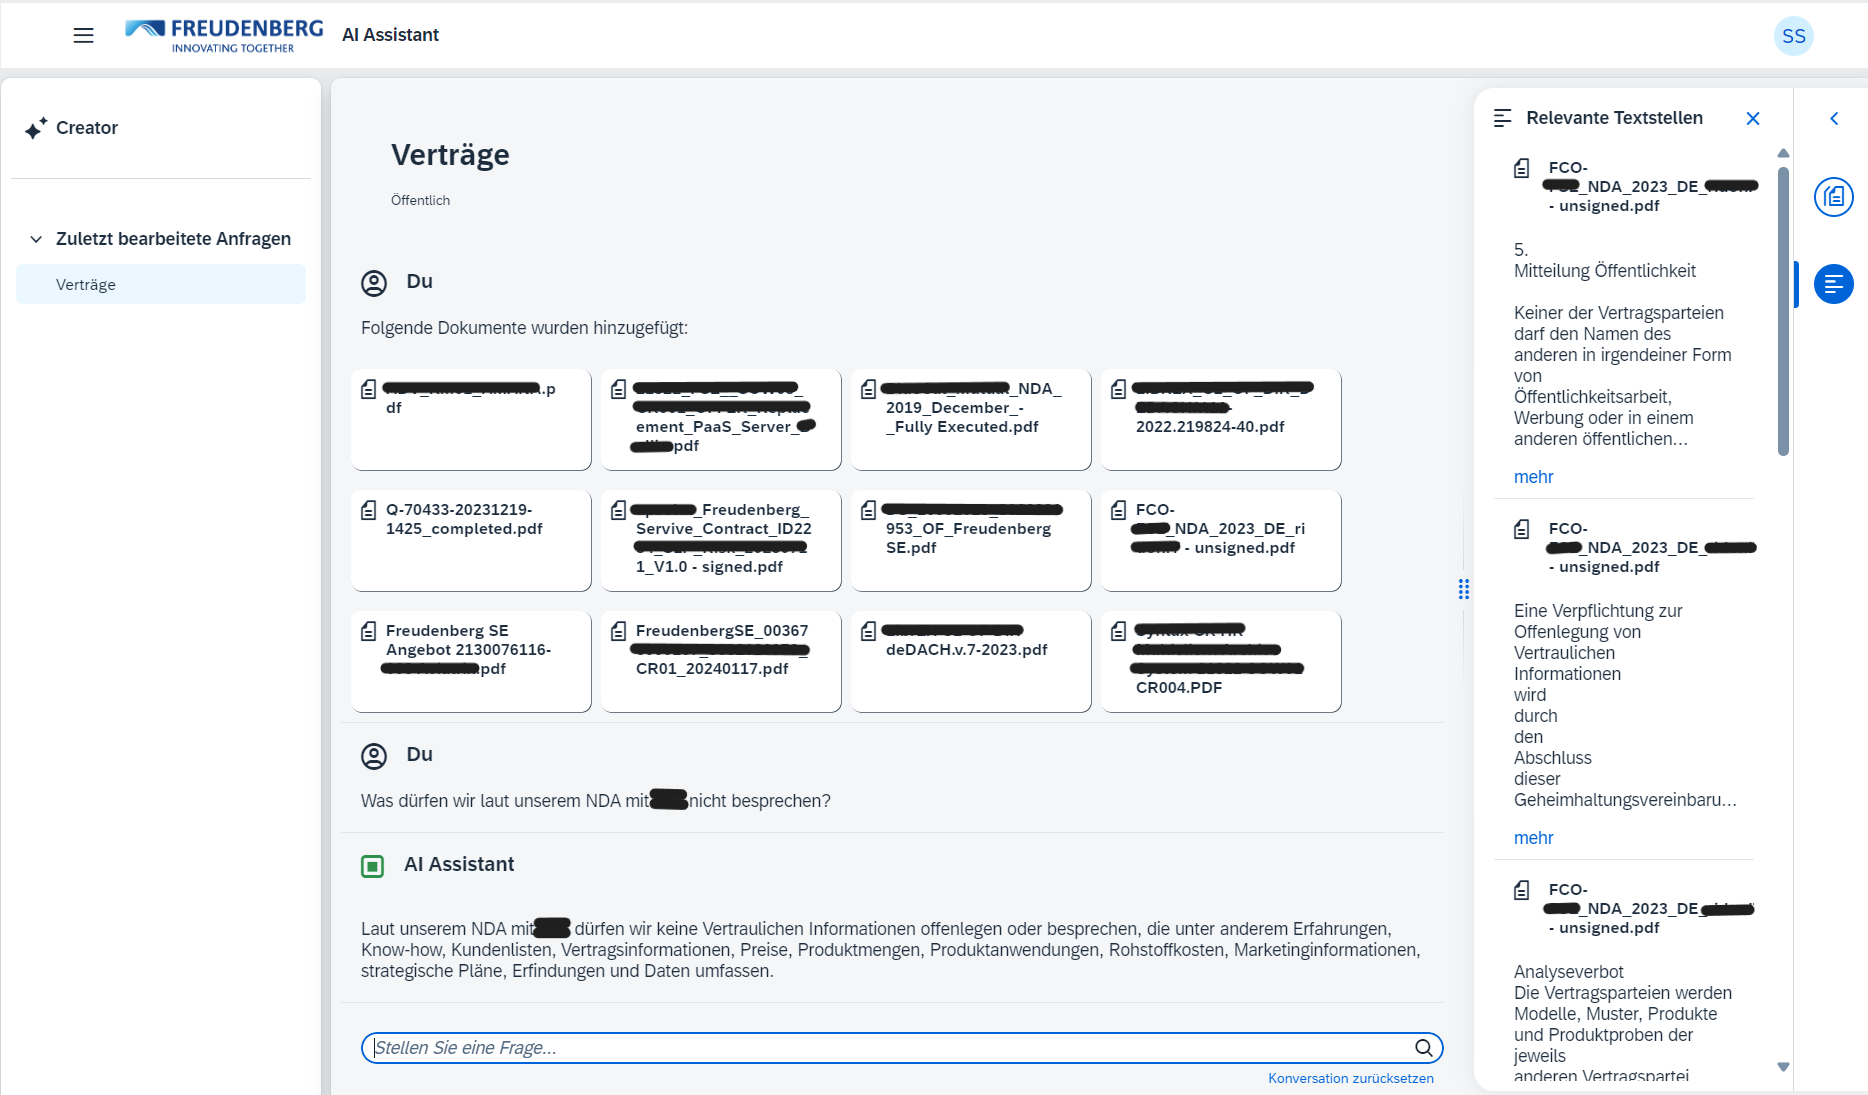
\includegraphics[width=1\textwidth]{img/Chatbot_vertraege_anfrage.png}
    \caption{Beispiel einer Anfrage zu Verträgen}
    \label{fig:chatbot_vertraege_anfrage}
\end{figure}

\subsection{Verlauf und Speicherfunktionalität}

Der AI Assistant kann zudem den gesamten Gesprächsverlauf für zukünftige Anfragen nutzen. In Abbildung \ref{fig:memory_proof} wird ein Beispiel gezeigt, 
in dem der Benutzer den Chatbot nach einem Angebot eines Vertragspartners fragt. Nachdem der Chatbot die Frage beantwortet hat, stellt der Benutzer eine neue Frage: „Was war nochmal meine Frage?“ 
Der Chatbot ist in der Lage, auf den Gesprächsverlauf zuzugreifen und korrekt zu antworten, indem er die ursprüngliche Frage wiedergibt. 
Dies wird ermöglicht, indem der gesamte Chatverlauf zur Laufzeit an das \ac{LLM} geschickt wird.

\begin{figure}[H]
    \centering
    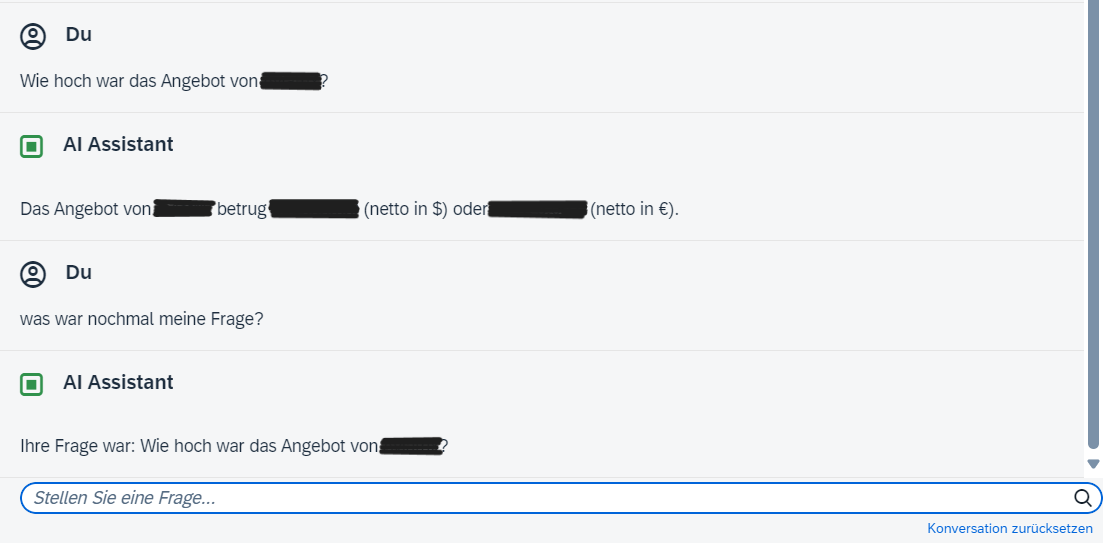
\includegraphics[width=1\textwidth]{img/Chatbot_memory_proof.png}
    \caption{Beweis für die Nutzung des Chatverlaufs}
    \label{fig:memory_proof}
\end{figure}

Zusätzlich wird in Abbildung \ref{fig:memory_use} ein weiteres Beispiel für die Gedächtnisfunktionalität gezeigt. Der Benutzer fragt den AI Assistant zuerst dieslbe Frage nach dem Angebot eines Vertragspartners 
und erhält dieselbe detaillierte Antwort. Anschließend stellt er eine Folgefrage: „Aus welchem Jahr?“ ohne das ursprüngliche Angebot erneut zu erwähnen. 
Der AI Assistant antwortet korrekt mit dem Jahr und dem exakten Datum des Angebots. Diese Funktionalität verbessert die Benutzerfreundlichkeit erheblich, 
da der Benutzer in der Lage ist, mehrere zusammenhängende Fragen zu stellen, ohne den gesamten Kontext wiederholen zu müssen. 
Dies ermöglicht präzisere und effizientere Konversationen, insbesondere bei komplexen Sachverhalten.

\begin{figure}[H]
    \centering
    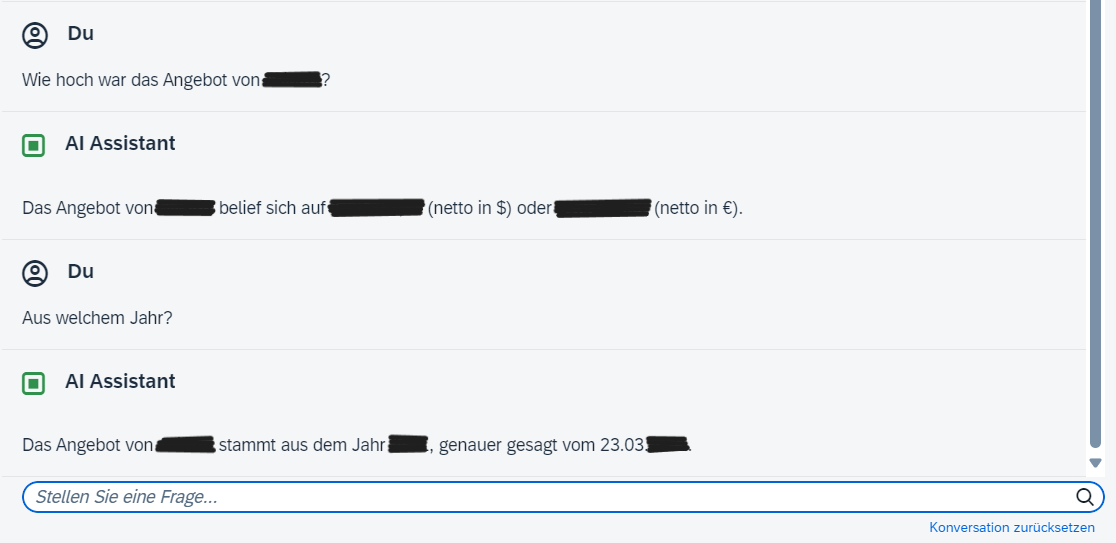
\includegraphics[width=1\textwidth]{img/Chatbot_memory_use.png}
    \caption{Nutzung des Chatverlaufs für präzisere Folgefragen}
    \label{fig:memory_use}
\end{figure}